{
  \newcommand\runtimeError{\begin{minipage}{0.03\textwidth}\centering\includegraphics[width=\linewidth]{Images/runtime-error}\end{minipage}}
  \newcommand\checkFailure{\begin{minipage}{0.03\textwidth}\centering\includegraphics[width=\linewidth]{Images/check-failure}\end{minipage}}
  \newcommand\blameFinger{\begin{minipage}{0.02\textwidth}\centering\vspace{0.25em}\includegraphics[width=\linewidth]{Images/finger}\end{minipage}}
  \newcommand\typeError{\scalebox{1.5}{$\tau_{\hspace{-0.1em}\times}$}}
  \newcommand\success{\textcolor{black!30!green}{\checkmark}}
  \newcommand\fail{\textcolor{red}{\sffamily x}}
  \footnotesize
\centering
\begin{tabular}{l|rcl|rcl|rc|c}
\multicolumn{7}{c}{\begin{minipage}{0.65\textwidth}\centering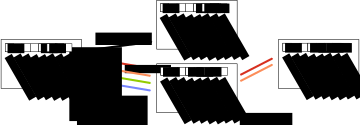
\includegraphics[width=\linewidth]{Images/trails-example}\end{minipage}} & %
\multicolumn{3}{c}{\begin{minipage}{0.25\textwidth}\centering\includegraphics[width=\linewidth]{Images/take5-module-graph}\end{minipage}} \\
\multicolumn{7}{c}{\begin{minipage}{0.65\textwidth}\centering The paths taken by each mode through the configuration lattice.\end{minipage}} & %
\multicolumn{3}{c}{\begin{minipage}{0.25\textwidth}\centering The module graph of take5.\end{minipage}}
\vspace{1em} \\
 & \textbf{Root} &  &  & \textbf{Step 1} &  &  & \textbf{Step 2} &  & \textbf{Success?}\\
\textbf{Mode} & config & result & stack & config & result & stack & config & result & \\
\hline
Natural & \textcolor{red}{1}000\textcolor{red}{1}\textcolor{red}{1}00 & \blameFinger & \texttt{main} & \textcolor{red}{1}000\textcolor{red}{1}\textcolor{red}{1}\textcolor{red}{1}0 & \typeError &  &  &  & \success\\
-blame &  & \texttt{player} & \texttt{main} &  &  &  &  &  & \\
\hline
Transient & \textcolor{red}{1}000\textcolor{red}{1}\textcolor{red}{1}00 & \runtimeError & \texttt{dealer} & \textcolor{red}{1}00\textcolor{red}{1}\textcolor{red}{1}\textcolor{red}{1}00 & \blameFinger & \texttt{dealer} & \textcolor{red}{1}00\textcolor{red}{1}\textcolor{red}{1}\textcolor{red}{1}\textcolor{red}{1}0 & \typeError & \success\\
-first-blame &  &  & \texttt{dealer} &  & \texttt{player} &  &  &  & \\
\emph{and} &  &  & \texttt{dealer} &  & \texttt{dealer} &  &  &  & \\
-last-blame &  &  & \texttt{main} &  &  &  &  &  & \\
\hline
Erasure & \textcolor{red}{1}000\textcolor{red}{1}\textcolor{red}{1}00 & \runtimeError & \texttt{dealer} & \textcolor{red}{1}00\textcolor{red}{1}\textcolor{red}{1}\textcolor{red}{1}00 & \runtimeError & \texttt{dealer} &  &  & \fail\\
 &  &  & \texttt{dealer} &  &  & \texttt{dealer} &  &  & \\
 &  &  & \texttt{dealer} &  &  & \texttt{dealer} &  &  & \\
 &  &  & \texttt{main} &  &  & \texttt{main} &  &  & \\
\hline
Natural & \textcolor{red}{1}000\textcolor{red}{1}\textcolor{red}{1}00 & \checkFailure & \texttt{main} &  &  &  &  &  & \fail\\
-exceptions &  &  & \texttt{main} &  &  &  &  &  & \\
\hline
Transient & \textcolor{red}{1}000\textcolor{red}{1}\textcolor{red}{1}00 & \runtimeError & \texttt{dealer} & \textcolor{red}{1}00\textcolor{red}{1}\textcolor{red}{1}\textcolor{red}{1}00 & \checkFailure & \texttt{dealer} &  &  & \fail\\
-exceptions &  &  & \texttt{dealer} &  &  &  &  &  & \\
 &  &  & \texttt{dealer} &  &  &  &  &  & \\
 &  &  & \texttt{main} &  &  &  &  &  & \\
\multicolumn{10}{c}{\begin{minipage}{0.95\textwidth}\vspace{0.5em} \textit{Legend.} Configurations: represented by a bit string, each digit corresponds to a module and indicates if it is typed. Results: \blameFinger~~denotes that the configuration results in a run-time type check failure blaming the module(s) below it, \checkFailure~~a run-time type check failure for which blame is ignored, \runtimeError~~an error from the runtime, and \typeError~~a type-checker error.\end{minipage}}  \\
\end{tabular}
}

